\documentclass[12pt, a4paper]{article}

%----------------------------------------------------------------------------------------
%	PACKAGES AND DOCUMENT CONFIGURATIONS
%----------------------------------------------------------------------------------------

\usepackage[utf8]{inputenc} % Input encoding
\usepackage[T1]{fontenc}    % Font encoding
\usepackage{lmodern}        % Moderne Schriftart
\usepackage{graphicx}       % Required for including images
\usepackage{amsmath}        % For advanced math environments
\usepackage{geometry}       % For page layout
\usepackage{csquotes}       % Empfohlen für biblatex
\geometry{a4paper, top=2.5cm, bottom=2.5cm, left=2.5cm, right=2.5cm}
\usepackage{hyperref}       % For hyperlinks and PDF metadata
\hypersetup{
    colorlinks=false,
    linkcolor=blue,
    filecolor=magenta,      
    urlcolor=cyan,
    pdftitle={My Study Work},
    pdfauthor={Your Name},
}

%----------------------------------------------------------------------------------------
%	Biblatex for Bibliography
%----------------------------------------------------------------------------------------
\usepackage[backend=biber, style=ieee, sorting=none]{biblatex}
\addbibresource{references.bib} % Your .bib file

%----------------------------------------------------------------------------------------
%	Header & Footer
%----------------------------------------------------------------------------------------
\usepackage{scrlayer-scrpage}
\pagestyle{scrheadings}
\automark{section}
\clearpairofpagestyles % Moderner Befehl statt \clearscrheadfoot
\ihead{\headmark} % Sektionsname oben innen
\cfoot{\pagemark} % Seitenzahl unten zentriert
\setkomafont{pageheadfoot}{\normalfont}


%----------------------------------------------------------------------------------------
%	Listings for Code Integration
%----------------------------------------------------------------------------------------
\usepackage{listings}
\usepackage{xcolor} % For custom colors in code

\definecolor{codegreen}{rgb}{0,0.6,0}
\definecolor{codegray}{rgb}{0.5,0.5,0.5}
\definecolor{codepurple}{rgb}{0.58,0,0.82}
\definecolor{backcolour}{rgb}{0.95,0.95,0.92}

\lstdefinestyle{cstyle}{
    backgroundcolor=\color{backcolour},   
    commentstyle=\color{codegreen},
    keywordstyle=\color{magenta},
    numberstyle=\tiny\color{codegray},
    stringstyle=\color{codepurple},
    basicstyle=\ttfamily\footnotesize,
    breakatwhitespace=false,         
    breaklines=true,                 
    captionpos=b,                    
    keepspaces=true,                 
    numbers=left,                    
    numbersep=5pt,                  
    showspaces=false,                
    showstringspaces=false,
    showtabs=false,                  
    tabsize=2,
    language=C
}
\lstset{style=cstyle}



%----------------------------------------------------------------------------------------
%	DOCUMENT START
%----------------------------------------------------------------------------------------

\begin{document}
%----------------------------------------------------------------------------------------
%	TITLE PAGE
%----------------------------------------------------------------------------------------

\begin{titlepage}
    \centering
    
    % \includegraphics[width=0.4\textwidth]{logo_thd.png} % Sie müssen eine Logo-Datei im Ordner haben
    
    \vspace{2cm}
    
    {\Huge\bfseries Ausarbeitung eines Konzepts für Ergonomische Arbeitsplätze einer Montagelinie\par}
    
    \vspace{1cm}
    
    {\Large Studienarbeit im Rahmen des AWP \\
    \enquote{Problemlösungen in der Praxis}\par}
    
    \vspace{2cm}
    
    {\large
    Vorgelegt von: \\
    \vspace{0.2cm}
    Felix Dick \\ 
    Matrikelnummer: 22111369 \\
    \vspace{1.5cm}
    
    Betreuer: \\
    Dipl.sc.pol.Univ., M.Sys.Eng. Roman Tizki \par} %
    
    \vfill % Füllt den vertikalen Raum
    
    {\large Deggendorf, den \today\par}

\end{titlepage}



\thispagestyle{empty}

\newpage

% --- Table of Contents ---
\tableofcontents
\newpage

%----------------------------------------------------------------------------------------
%	CHAPTERS
%----------------------------------------------------------------------------------------

\section{ANDi Tool and Loopback}
\label{sec:andi-tool}

This chapter introduces the initial setup and basic testing procedures.

\subsection{Introduction to the ANDI-tool}
% Describe the ANDI-tool, its purpose, and main features.
ANDi (Automotive Network Diagnoser ) is a cross-platform test and analysis tool for automotive electronic networks, designed to support software and ECU development at every stage. Its core functions are to simulate network traffic, execute component tests and analyse the resulting data\cite{technica}. It supports simulation, monitoring, and analysis of various network protocols, including CAN, LIN, FlexRay, and Ethernet (BroadR-Reach).
   
\subsection{Introduction to Wireshark}
Wireshark is a widely used open-source network protocol analyser. Its primary purpose is to capture and inspect data packets travelling across a network, enabling detailed analysis of network traffic. Key features include real-time packet capture, deep inspection of hundreds of protocols, filtering capabilities, and the ability to reconstruct data streams. 
   
\subsection{Loopback Test Procedure}
% Explain the steps to perform a loopback test. You can use an itemize or enumerate environment.
\begin{itemize}
    \item Step 1: Connect the hardware: Attach the ANDi device to the CAN bus or network interface intended for testing, ensuring all physical connections are secure and correct. 
    \item Step 2: Configure the software: Launch the ANDi software, set up the interface parameters (bitrate, channel, etc.), and enable loopback mode in the configuration settings. 
    \item Step 3: Run the test and observe results: Start the loopback test, send messages through the interface, and monitor received frames to verify correct transmission and reception within the same device. 
\end{itemize}

\subsection{Task Report}
The task utilized the ANDi tool in combination with Wireshark to establish communication through loopback testing. To achieve this, a stimulation and a logging adapter had to be selected. The stimulation adapter should transmit frames or signals, while the logging adapter is used to receive incoming packets.\\\\
After running a loopback script included in the task the packages were captured as expected, but only after selecting the right adapter for both (Figure 1). The layer 2 frame was received as expected (Figure 2) and could be traced in Wireshark.\\\\
\begin{figure}[h]
    \centering
     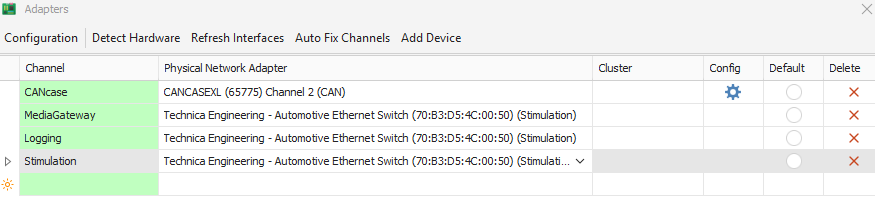
\includegraphics[width=0.8\textwidth]{figures/pictures/adaptersloopback.png}
    \caption{Selection of the same adapter for Logging and Stimulation.}
    \label{fig:mediagateway_setup}
\end{figure}
\begin{figure}[h]
    \centering
     
\includegraphics[width=0.8\textwidth]{figures/pictures/loopbackreceived.png}
    \caption{Received frame from loopback.}
    \label{fig:mediagateway_setup2}
\end{figure}
The next step was to create 2 distinct scripts, to distinguish between sending and receiving frames. Additionally the frames should be more distinguishable from another, so the requirement was to give each frame an identifier corresponding to the order they were sent in with 20 frames being sent over the course of 20 seconds.\\\\
After achieving this, subsequent task were to test further ANDi tools like SendPing and Burst Sending and analyze the traffic: Send Ping sends one request and awaits a reply while Burst Sending sends multiple requests in a short time without waiting for a reply first. Both operate on Layer 3 and use Ethernet frames on Layer 2 with the key difference being the number and timing of packets sent. \\\\
After changing the communication from Layer 2 (MAC address) to a layer 3 (IP address)  connection, the data frames change. They reveal more information about the connection, TTL, ports, and the checksum of the packages. 

\subsection{Conclusion}
In this package of Tasks basic understanding of packet construction and data traffic was developed by experimenting with a simulated point to point connection. The tasks were fairly basic and deepened the theoretical understanding of the topic, ensuring fundamental knowledge needed for subsequent tasks. No difficult challenges were encountered and the workflow was straightforward.

%To Do: Screenshots einfügen; 


\section{Part 2: ANDi Tool and Automotive Ethernet }
\label{sec:mediagateway}

This section details the establishment of a communication path.

\subsection{Simple Connection Setup}
% Describe the physical and logical setup for a simple connection. 
A simple setup typically means connecting two or more devices through the gateway, which acts as an intermediary for data transmission. For that devices are physically linked to the MediaGateway’s network ports using twisted pair cables and MediaConverters. The MediaGateway acts as a Layer 2 switch in this setup, forwarding Ethernet frames between connected devices without complex routing. Each device connects via its Ethernet port to a MediaConverter, which then connects to the MediaGateway. The gateway ports are set to slave mode by default, while the MediaConverters are configured as master. Logically, this setup establishes a direct Layer 2 link between the devices, allowing them to exchange Ethernet frames transparently through the MediaGateway.

\subsection{VLAN Configuration}
% Explain the concept of VLANs in this context and how to configure them.
VLANs (Virtual Local Area Networks) allow segmenting a physical network into multiple logical networks. In the context of the laboratory setup, VLANs create isolated broadcast domains within the MediaGateway, ensuring that only devices with matching VLAN tags can communicate with each other. Frames are tagged with a VLAN ID, and only those with a matching ID are forwarded within that VLAN. This improves bandwidth utilization and enhances security by isolating traffic, as frames without the correct VLAN tag cannot enter the VLAN and by thatunwanted access or interference is prevented.\\\\
To configure VLANs on the MediaGateway, you first assign VLAN IDs to internal ports and mark them as either tagged or untagged, depending on the connected device’s support. Since Windows does not support VLAN tagging natively, ports connecting to Windows devices are usually set as untagged members of a VLAN. Configuration is done via the MediaGateway’s web interface, where you enter the default IP address, enable IEEE 802.1Q VLAN mode, assign VLAN IDs to relevant ports, and then save and restart the gateway to apply the settings. After proper VLAN configuration, devices connected to the MediaGateway can communicate securely and efficiently within their assigned VLANs.\\\\
\begin{figure}[h]
    \centering
     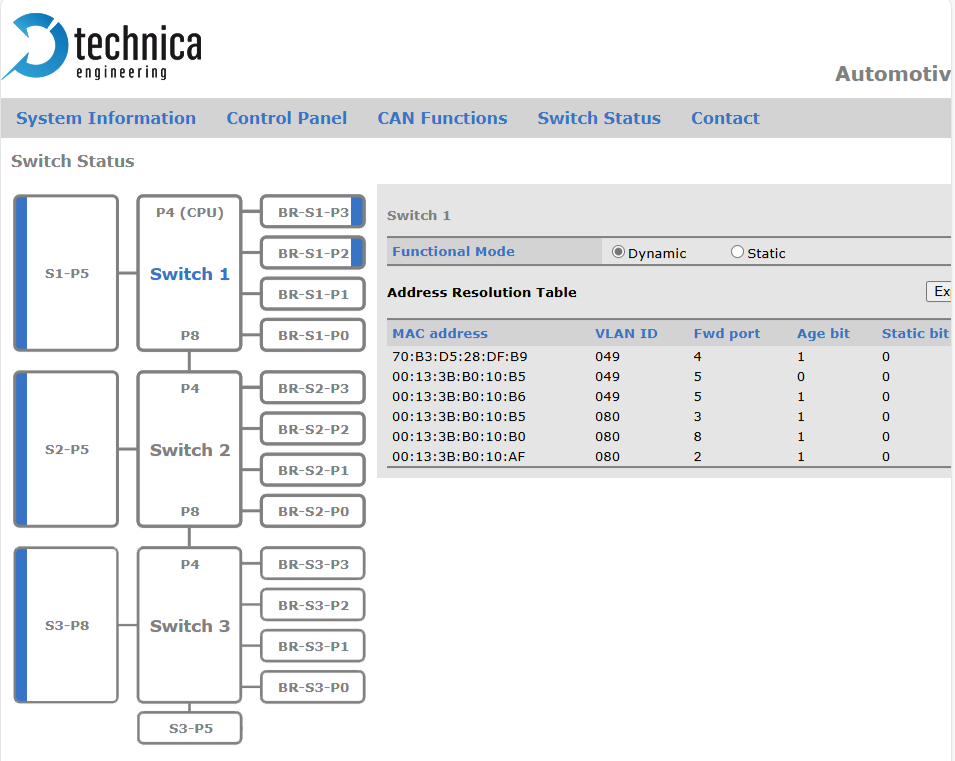
\includegraphics[width=0.8\textwidth]{figures/pictures/vlanconfig.PNG}
    \caption{VLAN Configuration.}
    \label{fig:mediagateway_setup3}
\end{figure}
\subsection{Task Report}
After realizing a simulated point to point connection in Part 1, this set of tasks revolved around advancing towards direct network communication through the Media Gateway with another physical workstation. The unconfigured media gateway will act as a layer 2 switch. Using the scripts from Part 1 as basis, they as well as the adapters had to be updated to reflect the new target.\\\\
The next task instructed the user to configure VLAN and build up a connection using it. Subsequently, a VLAN-based transmission path was configured, necessitating adjustments in the Media Gateway port settings (Figure 3). Upon correct VLAN implementation, packets containing payload data with increasing values were successfully transmitted and logged in Wireshark. The last task of this set, to access the webcam, was successful as well.\\\\
Significant challenges in this part included selecting the correct adapters and finding the correct port configuration, which was confusing at first, but after understanding the logic behind it, presented itself as a trivial matter. Another challenge was troubleshooting physical connectivity issues with an unresponsive webcam, which was later revealed to be the fault of a missing physical connection to the gateway.

\subsection{Conclusion}
In this package of Tasks the point to point connection to another workstation using the MediaGateway with the MAC address at first, then via VLAN-based transmission, was configured and established. The tasks helped further the understanding of VLAN and network traffic. There were some challenges in solving the tasks, but they were manageable to work around. 

%To Do: Screenshots einfügen; 





% A figure example:
%\begin{figure}[h]
    %\centering
    % \includegraphics[width=0.8\textwidth]{path/to/your/image.png}
    %\caption{Network diagram of the MediaGateway setup.}
    %\label{fig:mediagateway_setup}
%\end{figure}

\section{Part 3: ANDi Tool and Automotive Ethernet in the lab }
\label{sec:network-integration}

This chapter covers the integration of the setup into a larger network.

\subsection{Network Architecture Overview}
% Describe the target network architecture.
In Part 3 of the workshop, the target network architecture for integrating the setup consists of multiple workstations connected via individual MediaGateways to a central MediaGateway. Additionally, a webcam is connected to the central Gateway. Each workstation’s Gateway links through specific ports to the central gateway, creating a star-like topology. This central Gateway manages traffic between the different workstations and shared devices such as the central webcam, enabling communication beyond simple point-to-point connections. This architecture builds on the baseline established in earlier parts, where basic communication paths and VLAN configurations were performed between two devices over a single MediaGateway.

\subsection{Task Report}
The assigned tasks consisted of establishing a functional communication path between the workstation’s MediaGateway and the central MediaGateway, with the objective of accessing the central webcam. The process involved configuring each MediaGateway’s ports with the correct VLAN IDs and ensuring the physical connections to the central MediaGateway are correctly set up. \\\\
\begin{figure}[h]
    \centering
     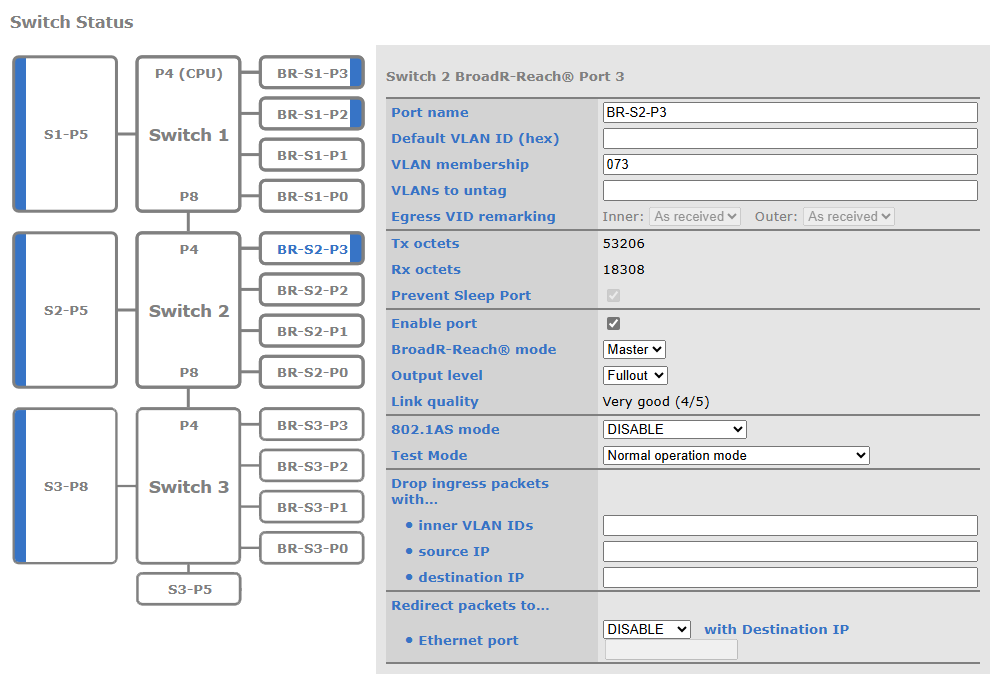
\includegraphics[width=0.8\textwidth]{figures/pictures/vlanconfig2.png}
    \caption{VLAN Configuration.}
    \label{fig:mediagateway_setup4}
\end{figure}\\ After setting up the configuration (Figure 4) a connection to the webcam could not be established, despite everything seemingly being correctly set up. The webcam stayed unresponsive to pings and even the instructor was unsure what was wrong. A restart of the central gateway and the central webcam was issued to troubleshoot, which solved the problem, despite the reason for the error staying unidentified. Post-reboot, connectivity was confirmed via successful ping responses. Remote access to the central webcam could be successfully established through a web browser . Concurrently, network traffic was captured using Wireshark, which verified the presence of correctly tagged Ethernet frames and validated the proper routing of data through the VLANs. 

\subsection{Conclusion}
In this package of Tasks the understanding of working with VLAN was deepened. The proficiency to solving the tasks profited from the gained understanding from prior parts. The unidentified error, that hindered progression of the task, was an obstacle that could be solved through the restart after a long period of tries to work around it.

%To Do: Screenshots einfügen; Netzwerkstruktur einfügen
\section{CAN-Ethernet-Gateway on Infineon AURIX TC297}
\label{sec:can-gateway}

This chapter focuses on the implementation of a CAN-Ethernet gateway.

\subsection{Hardware Overview: Infineon AURIX TC297}
% Describe the microcontroller and its relevant peripherals.
Placeholder for text...

\subsection{Software Implementation}
% Explain the software design and key algorithms.
Placeholder for text...

\subsubsection{C Code Example}
Here is an example of how to include a C code snippet.

\begin{lstlisting}[language=C, caption={Example of a simple CAN message sending function.}, label={lst:can_send}]
#include <stdio.h>

// Define CAN message structure
typedef struct {
    unsigned int id;
    unsigned char data[8];
    unsigned char dlc; // Data Length Code
} CAN_Message;

/*
 * @brief Sends a CAN message.
 * @param msg Pointer to the CAN_Message to be sent.
 */
void send_can_message(const CAN_Message* msg) {
    // Placeholder for actual hardware driver call
    printf("Sending CAN message with ID: 0x%X\n", msg->id);
    // ... implementation details for hardware registers ...
}

int main() {
    CAN_Message my_message;
    my_message.id = 0x123;
    my_message.dlc = 8;
    for (int i = 0; i < my_message.dlc; ++i) {
        my_message.data[i] = i;
    }
    
    send_can_message(&my_message);
    
    return 0;
}
\end{lstlisting}

%----------------------------------------------------------------------------------------
%	BIBLIOGRAPHY
%----------------------------------------------------------------------------------------

\newpage
\printbibliography[title={References}]

\end{document}